\title{Assignment 2 \\ \small{Evolutionary Computing}}
\author{Chiel ten Brinke 3677133}
\documentclass[12pt]{article}
\usepackage{amssymb,amsmath,amsthm,enumerate,graphicx,float,lmodern,xparse}
\usepackage{hyperref}

\usepackage{tabularx,ragged2e,booktabs,caption}
\usepackage[T1]{fontenc}
\usepackage[utf8]{inputenc}
\usepackage{tabularx,ragged2e,booktabs,caption}
\newcolumntype{C}[1]{>{\Centering}m{#1}}
\renewcommand\tabularxcolumn[1]{C{#1}}
\usepackage{changepage}
%\usepackage[showframe=true]{geometry}

\newtheorem{theorem}{Theorem}[section]
\newtheorem{lemma}[theorem]{Lemma}
\newtheorem{proposition}[theorem]{Proposition}
\newtheorem{corollary}[theorem]{Corollary}

\theoremstyle{definition}
\newtheorem{definition}[theorem]{Definition}
\newtheorem{axiom}[theorem]{Axiom}
\newtheorem{example}[theorem]{Example}
\newtheorem{remark}[theorem]{Remark}

\NewDocumentCommand\set{mg}{%
    \ensuremath{\left\lbrace #1 \IfNoValueTF{#2}{}{\, \middle|\, #2} \right\rbrace}%
}

\newcommand{\co}{\texttt{counting ones}}
\newcommand{\lsco}{\texttt{linearly scaled counting ones}}
\newcommand{\tdt}{\texttt{tightly linked deceptive trap}}
\newcommand{\tnt}{\texttt{tightly linked non-deceptive trap}}
\newcommand{\rdt}{\texttt{randomly linked deceptive trap}}
\newcommand{\rnt}{\texttt{randomly linked non-deceptive trap}}

\setcounter{secnumdepth}{3}

\begin{document}
\maketitle

\section*{Preliminary Notes}

\subsection*{Programming language}
The algorithms have been implemented in Cython~\cite{cython}.
Cython is a Python-like programming language which is translated into optimized
C/C++ code and compiled as Python extension modules.
This allows for very fast program execution, while keeping up the high programmer
productivity for which the Python language is well known.

We operate on 128 bit integers (GCC supports these), only using the first 100 bits.

\subsection*{Clustering Algorithm}
% Derive Jaccard distance from Mutual Information
% Refer to scipy

\subsection*{Experiments}
Since the implemention appears to be fast enough, the number of runs that is done to decide whether a population size is successful has been doubled.
So we consider problem to be solved reliably when 58 out of 60 independent runs find the optimal solution.

To get a better idea of how the population size influences the number of successes, we do not only show the population sizes that were used during the binary search, but with intervals of 20, we show the number of successes for each population size.

Nonetheless, the bisection search still has been implemented as required according to the instructions.
It has been used to determine the population size that is used to profile the fitness functions.

Other than the above, the assignment instructions have been followed precisely.
The obtained results can be found in the sections below.


\section{First Experiment}
\label{ssec:exp1}
In Figure~\ref{fig:exp1} the number of successes has been plot against the population size.
Table~\ref{tab:exp1} shows information concerning the fitness function evaluations.
Both randomly linked trap functions never reached an optimum, so they are not shown.

\begin{figure}[!htb]
    \centering
    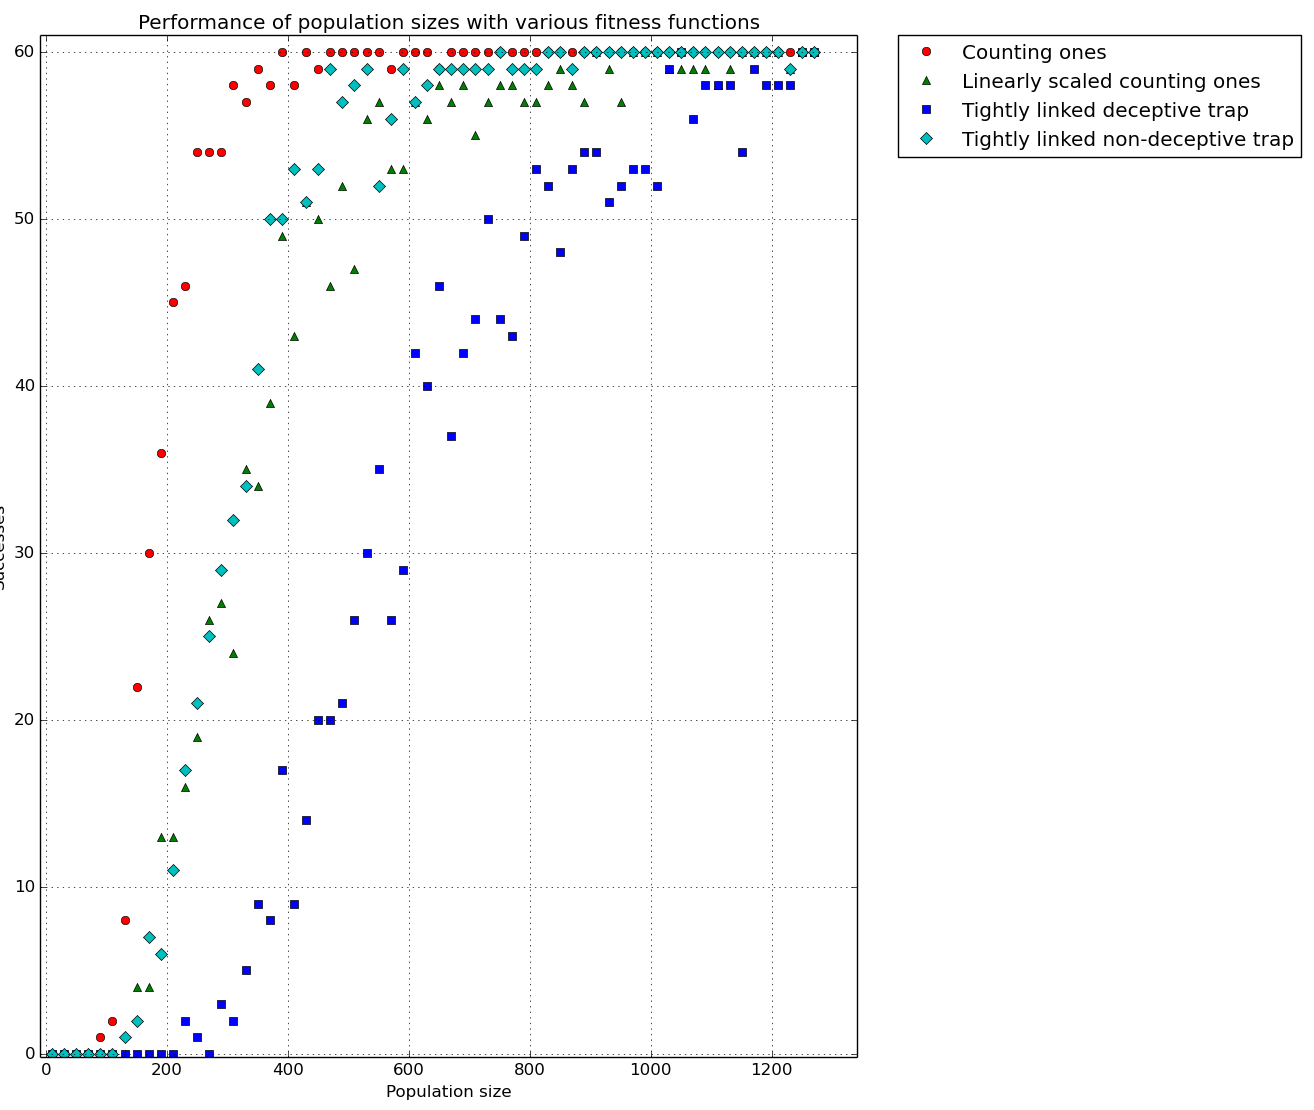
\includegraphics[totalheight=0.7\textheight]{images/exp1.png}
    \caption{Number of success per population size}
\label{fig:exp1}
\end{figure}

\begin{table}[!htb]
\begin{adjustwidth}{0cm}{}
\centering
\begin{tabular}{lp{2.5cm}p{2.5cm}p{2.8cm}}
\toprule[1.5pt]
\bf Fitness function & \bf Population size & \bf Function evaluations & \bf Corresponding CPU time\\\midrule
Counting ones & 310 & 51094 & 0.013 seconds \\
Linearly scaled Counting ones & 730 & 164174 & 0.030 seconds \\
Tightly linked deceptive trap & 1210 & 243142 & 0.429 seconds \\
Tightly linked non-deceptive trap & 610 & 93278 & 0.177 seconds \\
\bottomrule[1.25pt]
\end{tabular}\par
\bigskip
\captionof{table}{Fitness function evaluations}
\label{tab:exp1}
\end{adjustwidth}
\end{table}

% Constructs: to be expected, intuitively clear, not surprising, evident
\paragraph{Observations}
% two-point crossover is bad for randomly linked trap functions
The first observation one can make is that randomly linked trap functions never reach an optimum with population sizes lower than 1280.
This is not surprising since the two-point crossover can't flip multiple bits
in random places at the same time, which is important to improve subfunctions to their best state.
Unless the optimum is generated by accident at a very early stage of the evolution
(the probability of this happening is very small for the population sizes we've tried),
0s will soon dominate a lot of bit positions.
Since the two point crossover can't turn them into ones, an optimum will never be found.


\begin{thebibliography}{9}

\bibitem{cython}
R. Bradshaw, S. Behnel, D. S. Seljebotn, G. Ewing, et al.,
The Cython compiler, \url{http://cython.org}.

\end{thebibliography}


\end{document}
